\section{Improved Hyperparameter Tuning} \label{sec-hyperparam-optimization}
Hyperparameters of a machine learning model greatly impact on the quality of the model.
There are three common techniques for tuning the hyperparameters, namely, grid search, random search, and Bayesian hyperparameter search \cite{hutter2011sequential,snoek2012practical}.
In this section, we propose three optimizations to improve the process of hyperparameter tuning.

\subsection{Search unpacking}
Existing machine learning libraries provide black-box operations for performing the hyperparameter tuning operation.
However, every search process only consists of a series of individual training operations that only differ in hyperparameters.
Therefore, instead of using black-box operations, we consider each training run in the hyperparameter tuning process as a separate operation.
As a result, we consider each training run a separate workload, where we try to utilize the reuse and warmstarting operations when possible.
\todo[inline]{Do we need a figure for clarification?}
%To optimize the grid and random search operation, we first transform them into several model training operations through a simple process called grid unpacking.
%In grid unpacking, each training operation is considered a separate workload.
%Figure \ref{fig-grid-unpacking} shows an example of grid unpacking for a simple SVM Model which has the two hyperparameters penalty (C) and learning rate.
%After unpacking, the reuse optimizations techniques discussed in Section \ref{sec-reuse-and-warmstarting} can be applied.
%\begin{figure}
%\centering
%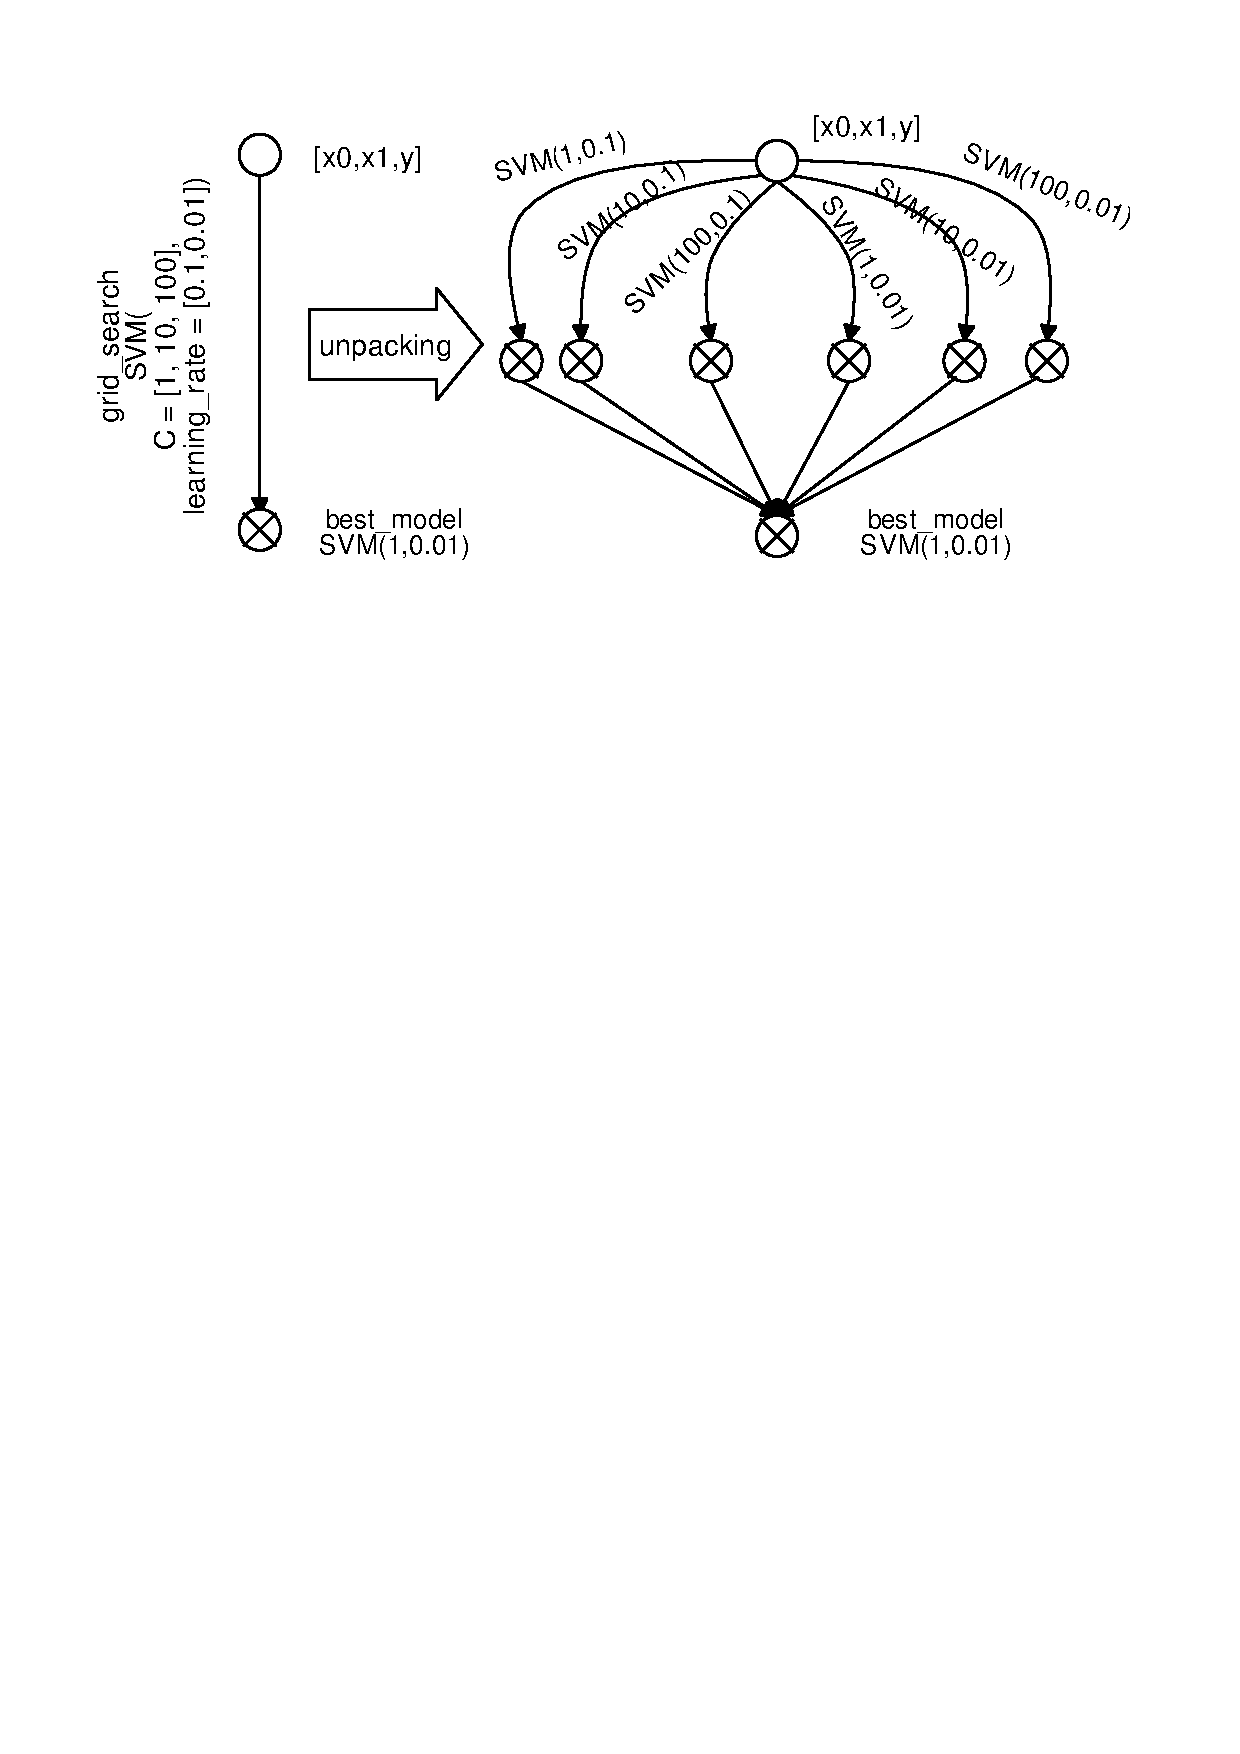
\includegraphics[width=\columnwidth]{../images/grid-unpacking}
%\caption{Result of unpacking on a small grid for SVM model. The hyperparameters are C=[1, 10, 100] and learning rate=[0.1, 0.01]}
%\label{fig-grid-unpacking}
%\end{figure}

\subsection{Automatic Search Space Definition}\label{sub-section-automatic-search-definition}
A major challenge in all the hyperparameter tuning techniques is defining the appropriate search space.
Currently, the ranges of the hyperparameters are defined through trial-and-error, experience, and common sense.
We propose to extract the hyperparameter ranges from the experiment database.
These extracted values can guide us to define the search space over the hyperparameters.
As a result, the search process becomes less challenging for users, especially the users that do not have in-depth knowledge of machine learning.
We utilize the performance of the model (quality metric) to specify a goodness measure for the value of the hyperparameters.
This helps us to discover the promising (and unpromising) regions for the hyperparameters.
\todo[inline]{If we end up including AutoML as well, we should mention again that hyperparameters are not just limited to models anymore and any pipeline design decision counts as a (possible) hyperparameter}

\subsubsection{Explorer unit}
One problem when defining the search space having few instances for some specific hyperparameters.
To address this issue, we design a component called the explorer unit.
After a workload is executed, we first determine if there are similar workloads in the experiment database.
Similar workloads are defined workloads that operate on the same dataset.
In case the number of the similar workloads is below a threshold, we invoke the explorer unit to automatically propose values for hyperparameters and find the performance of the model trained using each hyperparameter setting.
%\todo[inline]{This can be defined as a combination of the existing 'best-practices' and a random walk}

\subsection{Fast Bayesian Hyperparameter Tuning and AutoML}
One drawback of the Bayesian hyperparameter tuning is that it requires many initial random trials until it starts to propose promising hyperparameters \cite{hutter2011sequential,snoek2012practical}.
By utilizing the experiment database, we devise a strategy to decrease the number of initial trials (or in some cases avoid it altogether).
As a result, the search process can propose promising hyperparameters faster.

Our solution is as follows.
For every existing model group in the experiment database, we start a Bayesian search process.
A model group is a set of models that only differ in their hyperparameter values.
We then initialize the search process by including the existing hyperparameters and the corresponding model quality from the model group.
For every new workload, we transform it into its graph representation.
We anticipate three types of workloads.
In the first type, the workload may contain a model training operation with all of the hyperparameters already set.
In this case, we only execute the model training operation with the given hyperparameters and return the model (no optimization).
In the second type, the workload does not contain the hyperparameter values, and the user relies on our hyperparameter search to receive promising hyperparameters.
In this case, we first find the model group that this workload belongs to.
Then, from the corresponding Bayesian search process, we utilize the proposed hyperparameters to train the model.
In the third type, a user may specify a Bayesian search process with a specific budget \textit{within} the workload.
In this case, similar to the second workload type, we find the corresponding Bayesian search process and resume the Bayesian hyperparameter search until the budget is exhausted.
\todo[inline]{should we do AutoML in this paper}
Next, we plan to extend the Bayesian hyperparameter search to the entire pipeline, typically referred to as AutoML \cite{thornton2013auto}.
In AutoML, the decision to perform an operation on the training dataset is also considered a hyperparameter.
As a result, we can propose a promising machine learning \textit{pipelines} instead of just hyperparameters for the model.

%\subsubsection{Avoiding Local Optima}
%\todo[inline]{This may not be a problem though. I can find out more after running some more experiments.}
%Warm starting for hyperparameter optimization and AutoML have the benefit of reducing the overhead of computing many trials.
%However, inserting the data from the experiment database into the optimization process may lead the search into local optima.
%This could decrease the chance of finding the best hyperparameter setting.
%However, our automatic search space definition mechanism alleviates this problem as it explores the regions beyond what is currently defined in the experiment database.
%Furthermore, we propose a simple \textit{adaptive warmstarting} method that chooses promising points.